\documentclass{standalone}

\usepackage{tikz}
\usetikzlibrary{decorations.markings}
\usetikzlibrary{arrows.meta}
\usetikzlibrary{calc}

\usepackage{amsmath}

\begin{document}


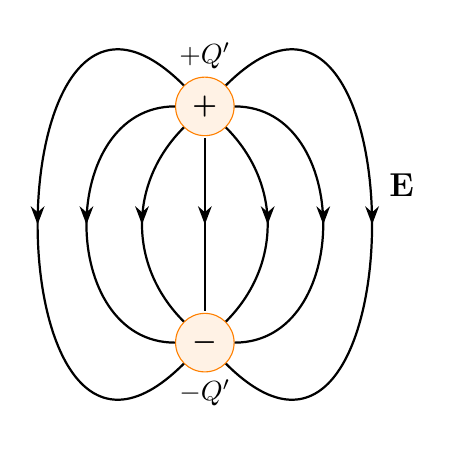
\begin{tikzpicture}[baseline=(current bounding box.south)]

% Define styles
\tikzset{
    charge/.style={fill=orange!10, draw=orange, circle, radius=0.4},
    fieldline/.style={thick, postaction={decorate}, decoration={markings}},
    arrow/.style={decoration={mark=at position #1 with {\arrow{Stealth}}}},
    reversearrow/.style={decoration={mark=at position #1 with {\arrowreversed{Stealth}}}}
}


% zeige den Teil, der durch die Graphik benutzt wird
\useasboundingbox (2.75,2) rectangle (7.75,7);


% grind lines
%\draw[help lines, dashed] grid (10,10);

%position of bottom wire
\coordinate (A1) at (5,3);

%position of top wire
\coordinate (A2) at (5,6);

% Negative charge node
\node[draw=orange, fill=orange!10, circle] (NEG) at (A1) {$\boldsymbol{-}$};
\node[below=1em] at (NEG) {$-Q^{\prime}$};


% Positive charge node
\node[draw=orange, fill=orange!10, circle] (POS) at (A2) {$\boldsymbol{+}$};
\node[above=1em] at (POS) {$+Q^{\prime}$};


% Electric field lines
\draw[fieldline, arrow=0.5] ($(A2)+(0.0,-0.4)$) -- ($(A1)+(0,0.4)$);



\draw[fieldline, arrow=0.5] (node cs:name=POS, angle=-45) .. controls +(-45:1) and +(45:1) .. (node cs:name=NEG,
angle=45);

\draw[fieldline, arrow=0.5] (node cs:name=POS, angle=-135) .. controls +(-135:1) and +(135:1) .. (node cs:name=NEG,
angle=135);



\draw[fieldline, arrow=0.5] (node cs:name=POS, angle=0) .. controls +(0:1.5) and +(0:1.5) .. (node cs:name=NEG,
angle=0);

\draw[fieldline, arrow=0.5] (node cs:name=POS, angle=180) .. controls +(180:1.5) and +(180:1.5) .. (node cs:name=NEG,
angle=180);



\draw[fieldline, arrow=0.5] (node cs:name=POS, angle=45) .. controls +(45:3.5) and +(-45:3.5) .. (node cs:name=NEG,
angle=-45);

\draw[fieldline, arrow=0.5] (node cs:name=POS, angle=135) .. controls +(135:3.5) and +(-135:3.5) .. (node cs:name=NEG,
angle=-135);



% Electric field label
\node at (7.5,5) {\large \textbf{E}};

\end{tikzpicture}


\end{document}